Gli idrocarburi policiclici aromatici (IPA) vengono comunemente ricercati nel PM10 data la loro tossicità; per uno di essi, il benzo(a)pirene (BaP), sussiste inoltre il limite legale di $1 ng/m^3$ come media annua. Questi inquinanti originano da processi di combustione fra cui si rammentano il traffico veicolare e il riscaldamento domestico. In regione sono molte le stazioni dedicate a questo tipo di indagine in quanto le medie annue di BaP risultano, ancorché entro il limite di $1 ng/m^3$, spesso al di sopra della soglia di valutazione superiore.

Sono state analizzate le concentrazioni degli IPA campionati in 3 stazioni in provincia di Udine: la stazione di fondo urbano di Udine centro (v. Cairoli), la stazione urbana di montagna di Tolmezzo e la stazione suburbana di montagna di Ugovizza. Essendo gli IPA una tipologia di inquinanti dovuta alla combustione, e di natura prevalentemente invernale (sia per la maggiore presenza di fonti di emissione come il riscaldamento domestico, sia per la natura chimica e fotochimica di questi composti), il mese di marzo registra solitamente concentrazioni abbastanza basse di questi analiti, spesso vicini al limite di rilevazione strumentale (LOQ). Per questo motivo, l’analisi viene effettuata su “cumuli” di filtri giornalieri, al fine di raggiungere in ciascuna analisi una quantità di inquinante analiticamente apprezzabile. I campioni del mese di marzo sono stati quindi “cumulati” su questi periodi: 
\begin{itemize}
    \item 1--13/3, prima del \textit{lockdown} (“tr ON” nei grafici);
    \item 14--26/3, durante il \textit{lockdown} (“tr OFF”);
    \item 27--29/3, durante l'evento di trasporto di polveri desertiche ("dust");
    \item 30--31/3 ("norm").
\end{itemize}

\begin{figure}
    \centering
    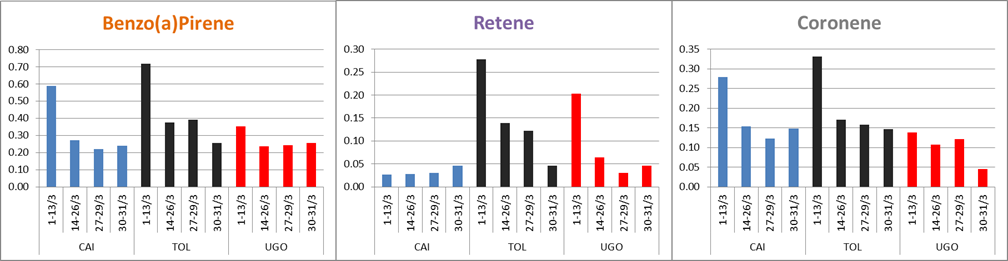
\includegraphics[width=\textwidth]{figs/ipa-barre.png}
    \caption[Concentrazioni in atmosfera di BaP, retene e coronene]{Concentrazioni in atmosfera (in $ng/m^3$) dei tre IPA benzo(a)pirene, retene e coronene, nei tre siti di Udine CAI, Tolmezzo TOL e Ugovizza UGO.}
    \label{fig:ipa2}
\end{figure}

Il \textit{lockdown} ha dunque impatti diversi sui tre IPA benzo(a)pirene, retene e coronene (fig.\ref{fig:ipa2}). Il confronto tra i primi 13 giorni del mese e le giornate seguenti lo evidenzia. Il retene (origine: combustione di legna resinosa) risulta sostanzialmente assente nella stazione urbana di Udine, mentre gli altri composti, ampiamente presenti nel sito, risentono del \textit{lockdown}. Le concentrazioni di benzo(a)pirene e coronene sono sostanzialmente dimezzate (rispetto ai primi 13 giorni del mese) in tutte le stazioni tranne quella di Ugovizza: in quest’ultima stazione l’entità del decremento è minore, a testimonianza del minore impatto della fonte traffico su quel sito.

\begin{figure}
    \centering
    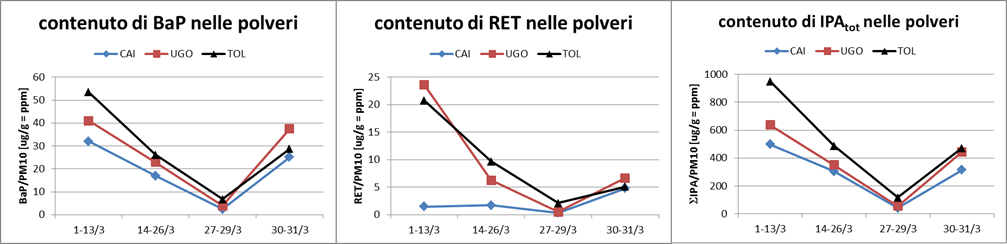
\includegraphics[width=\textwidth]{figs/ipa-linee.png}
    \caption[Concentrazioni nel PM10 di BaP, retene e IPA totali]{Concentrazioni nel PM10 di BaP, retene e IPA totali, nei tre siti di Udine CAI, Tolmezzo TOL e Ugovizza UGO.}
    \label{fig:ipa3}
\end{figure}

Se le sostanze aerodisperse vengono riferite, anziché al metro cubo d’aria, alla concentrazione di PM10 effettivamente presente in quello stesso metro cubo d’aria, si nota come il contenuto di BaP e di IPA totali nelle polveri (\ref{fig:ipa3}, primo e terzo pannello), diminuisce con il \textit{lockdown}, ed ancor più durante il successivo episodio di polveri desertiche. Nelle ultime giornate del mese, il contenuto di IPA torna a livelli del tutto simili a quelli del primo periodo di \textit{lockdown}.

\begin{figure}
    \centering
    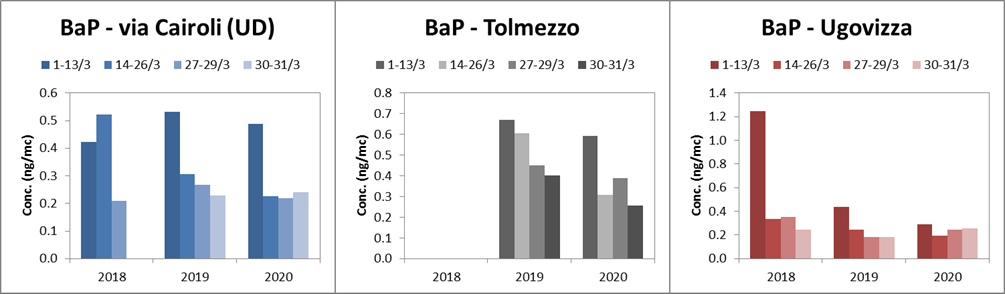
\includegraphics[width=\textwidth]{figs/bap-barre.png}
    \caption{Concentrazioni di BaP a marzo 2020, confronto con i due anni precedenti}
    \label{fig:ipa4}
\end{figure}
\begin{figure}
    \centering
    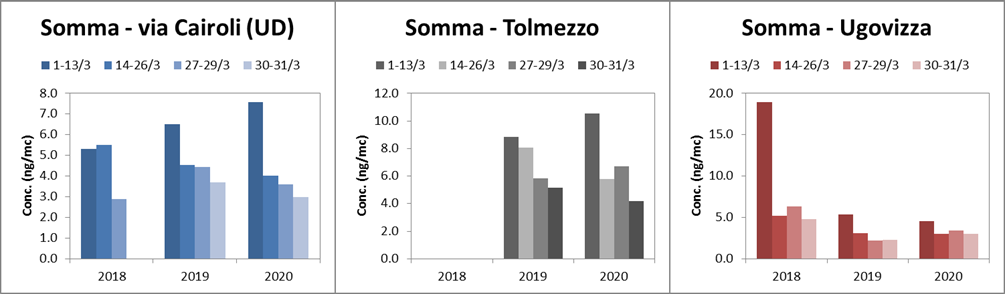
\includegraphics[width=\textwidth]{figs/ipa-somma-barre.png}
    \caption{Concentrazioni di IPA totali a marzo 2020, confronto con i due anni precedenti}
    \label{fig:ipa5}
\end{figure}

Come per altri inquinanti, la difficoltà nel trarre conclusioni definitive sugli effetti del \textit{lockdown} deriva dal fatto che esso si è verificato in un mese di transizione tra una stagione fredda e una più mite. Le figure \ref{fig:ipa4} e \ref{fig:ipa5} evidenziano come anche nei due anni precedenti si sia registrata una netta variazione nell'arco del mese. Tuttavia, nella stazione di Udine la variazione è stata decisamente più marcata che in passato. Ciò suggerisce che il \textit{lockdown} abbia avuto un impatto sugli IPA più marcato nelle aree maggiormente urbanizzate.

Per superare in qualche misura le limitazioni di queste analisi univariate, si è realizzata un'analisi multivariata, tenendo in considerazione contemporaneamente tutti i congeneri IPA analizzati. Si è condotta un’Analisi delle Componenti Principali PCA, \citep{wold1984multivariate}, riportando nel piano delle prime due Componenti Principali sia la proiezione dei campioni che quella delle variabili chimiche originali: si ottiene cioè il \textit{biplot}\footnote{varianza spiegata dal biplot: 92\%, di cui varianza spiegata dalla prima componente principale (PC1, asse orizzontale): 83\%; varianza spiegata dalla PC2 (asse verticale): 10\%.} riportato in figura \ref{fig:ipa1}.

Poiché i \textit{loadings} di quasi tutti i congeneri IPA sono orientati verso i due quadranti di destra (cioè sul verso positivo della PC1), mentre quello del retene (“RET” nel grafico\footnote{il retene è un alchil-IPA derivante dalla combustione dell’acido abietico contenuto nelle resine delle conifere}), risulta orientato verso il basso, a differenza della maggior parte degli altri congeneri, è possibile identificare la PC1 (asse orizzontale) come una componente che rendiconta la generale intensità dell’impatto degli IPA, e la PC2 come una componente che discrimina tra la fonte traffico e la fonte da combustione di biomassa (\textit{biomass burning}). 
Dunque i campioni a maggior impatto complessivo da IPA si collocano a destra nel grafico, quelli a minor impatto da IPA a sinistra; i campioni a prevalente fonte traffico si collocano in alto, mentre quelli a prevalente fonte \textit{biomass burning} si collocano in basso.

La transizione dal periodo pre-\textit{lockdown} ("tr ON" nel \textit{biplot}) al periodo di \textit{lockdown} ("tr OFF") è differente per le tre stazioni: 
\begin{itemize}
    \item a Udine si registra un netto spostamento dalla zona ad alto impatto di IPA di origine traffico a quella a basso impatto di IPA; 
    \item anche a Tolmezzo il \textit{lockdown} determina una netta attenuazione dell'impatto da IPA, ma rispetto a Udine il contributo della combustione di legna è più marcato, e durante il blocco risulta prevalente;
    \item infine a Ugovizza l'impatto degli IPA è molto minore, soprattutto ascrivibile alla combustione di biomassa legnosa, e non significativamente alterato dal \textit{lockdown}.
\end{itemize}

\begin{landscape}
\begin{figure}
    \centering
    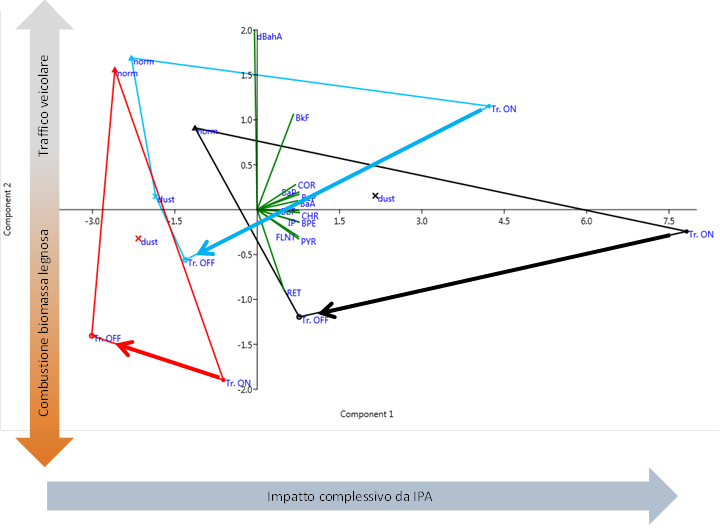
\includegraphics[width=0.9\linewidth]{figs/ipa-pca.png}
    \caption[PCA degli IPA a Udine, Tolmezzo e Ugovizza]{PCA degli IPA a Udine (azzurro), Tolmezzo (nero) e Ugovizza (rosso). I vettori in verde rappresentano le proiezioni degli assi relativi alle variabili chimiche originali (\textit{loadings}). Le etichette blu individuano i quattro periodi di campionamento: "tr ON" 1--13/3, "tr OFF" 14--26/3, "dust" 27--29/3, "norm" 30--31/3. Le frecce più spesse individuano la transizione da pre-\textit{lockdown} a \textit{lockdown}.}
    \label{fig:ipa1}
\end{figure}
\end{landscape}
